\documentclass[nochap]{apuntes}

\title{Hoja 3 Autómatas y Lenguajes}
\author{Víctor de Juan Sanz}
\date{2014}


\begin{document}
\maketitle
\section{Análisis sintáctico ascendente}

\begin{problem}[1]
Sea la siguiente gramática:
\begin{align*}
(1)\quad & S ::= A\\
(2)\quad & S ::= B\\
(3)\quad & A ::= cA + b\\
(4)\quad & A ::= a\\
(5)\quad & B ::= cB + a\\
(6)\quad & B ::= b
\end{align*}
Calcula los conjuntos primero y siguiente para cada símbolo no terminal.

\solution

\subparagraph{Primero(A): } {c,a}
\subparagraph{Siguiente(A) : } {\$,+}

\subparagraph{Primero (B):} {c,b}
\subparagraph{Siguiente (B): } {\$,+}

\subparagraph{Primero (S):} {a,b,c}
\subparagraph{Siguiente (S): } {\$}
\end{problem}


\begin{problem}[2]
Sea la siguiente gramática LR(0):
\begin{align*}
(1) & E ::= T\\
(2) & E ::= E + T\\
(3) & T ::= i\\
(4) & T ::= (E)
\end{align*}

Calcula el cierre de la configuración inicial E’ ::= .E\$

\solution
\begin{align*}
E' &::= .E\$\\
E &::= .E + T\\
E &::= .T\\
T &::= .i\\
T &::= .(E)
\end{align*}
\end{problem}


\begin{problem}[3]
\ppart Calcula el cierre de la configuración E ::= (.L)

\ppart Calcula el estado al que se llega desde el estado anterior tras reconocer el símbolo no terminal L.
\solution

\spart
\begin{align*}
E ::= (.L)\\
L ::= .L,E\\
L ::= .E\\
E ::= .i\\
E :: = .(L)
\end{align*}
\spart

\begin{align*}
L ::= (L.)
\end{align*}
\end{problem}

	
\begin{problem}[4]

\ppart Dibuja el diagrama de estados del analizador LR(0) para dicha gramática.
\ppart Calcula la tabla de análisis para el analizador LR(0).
\ppart Indica justificadamente si la gramática es LR(0). Indica justificadamente si es
SLR(1).
\solution

\spart 
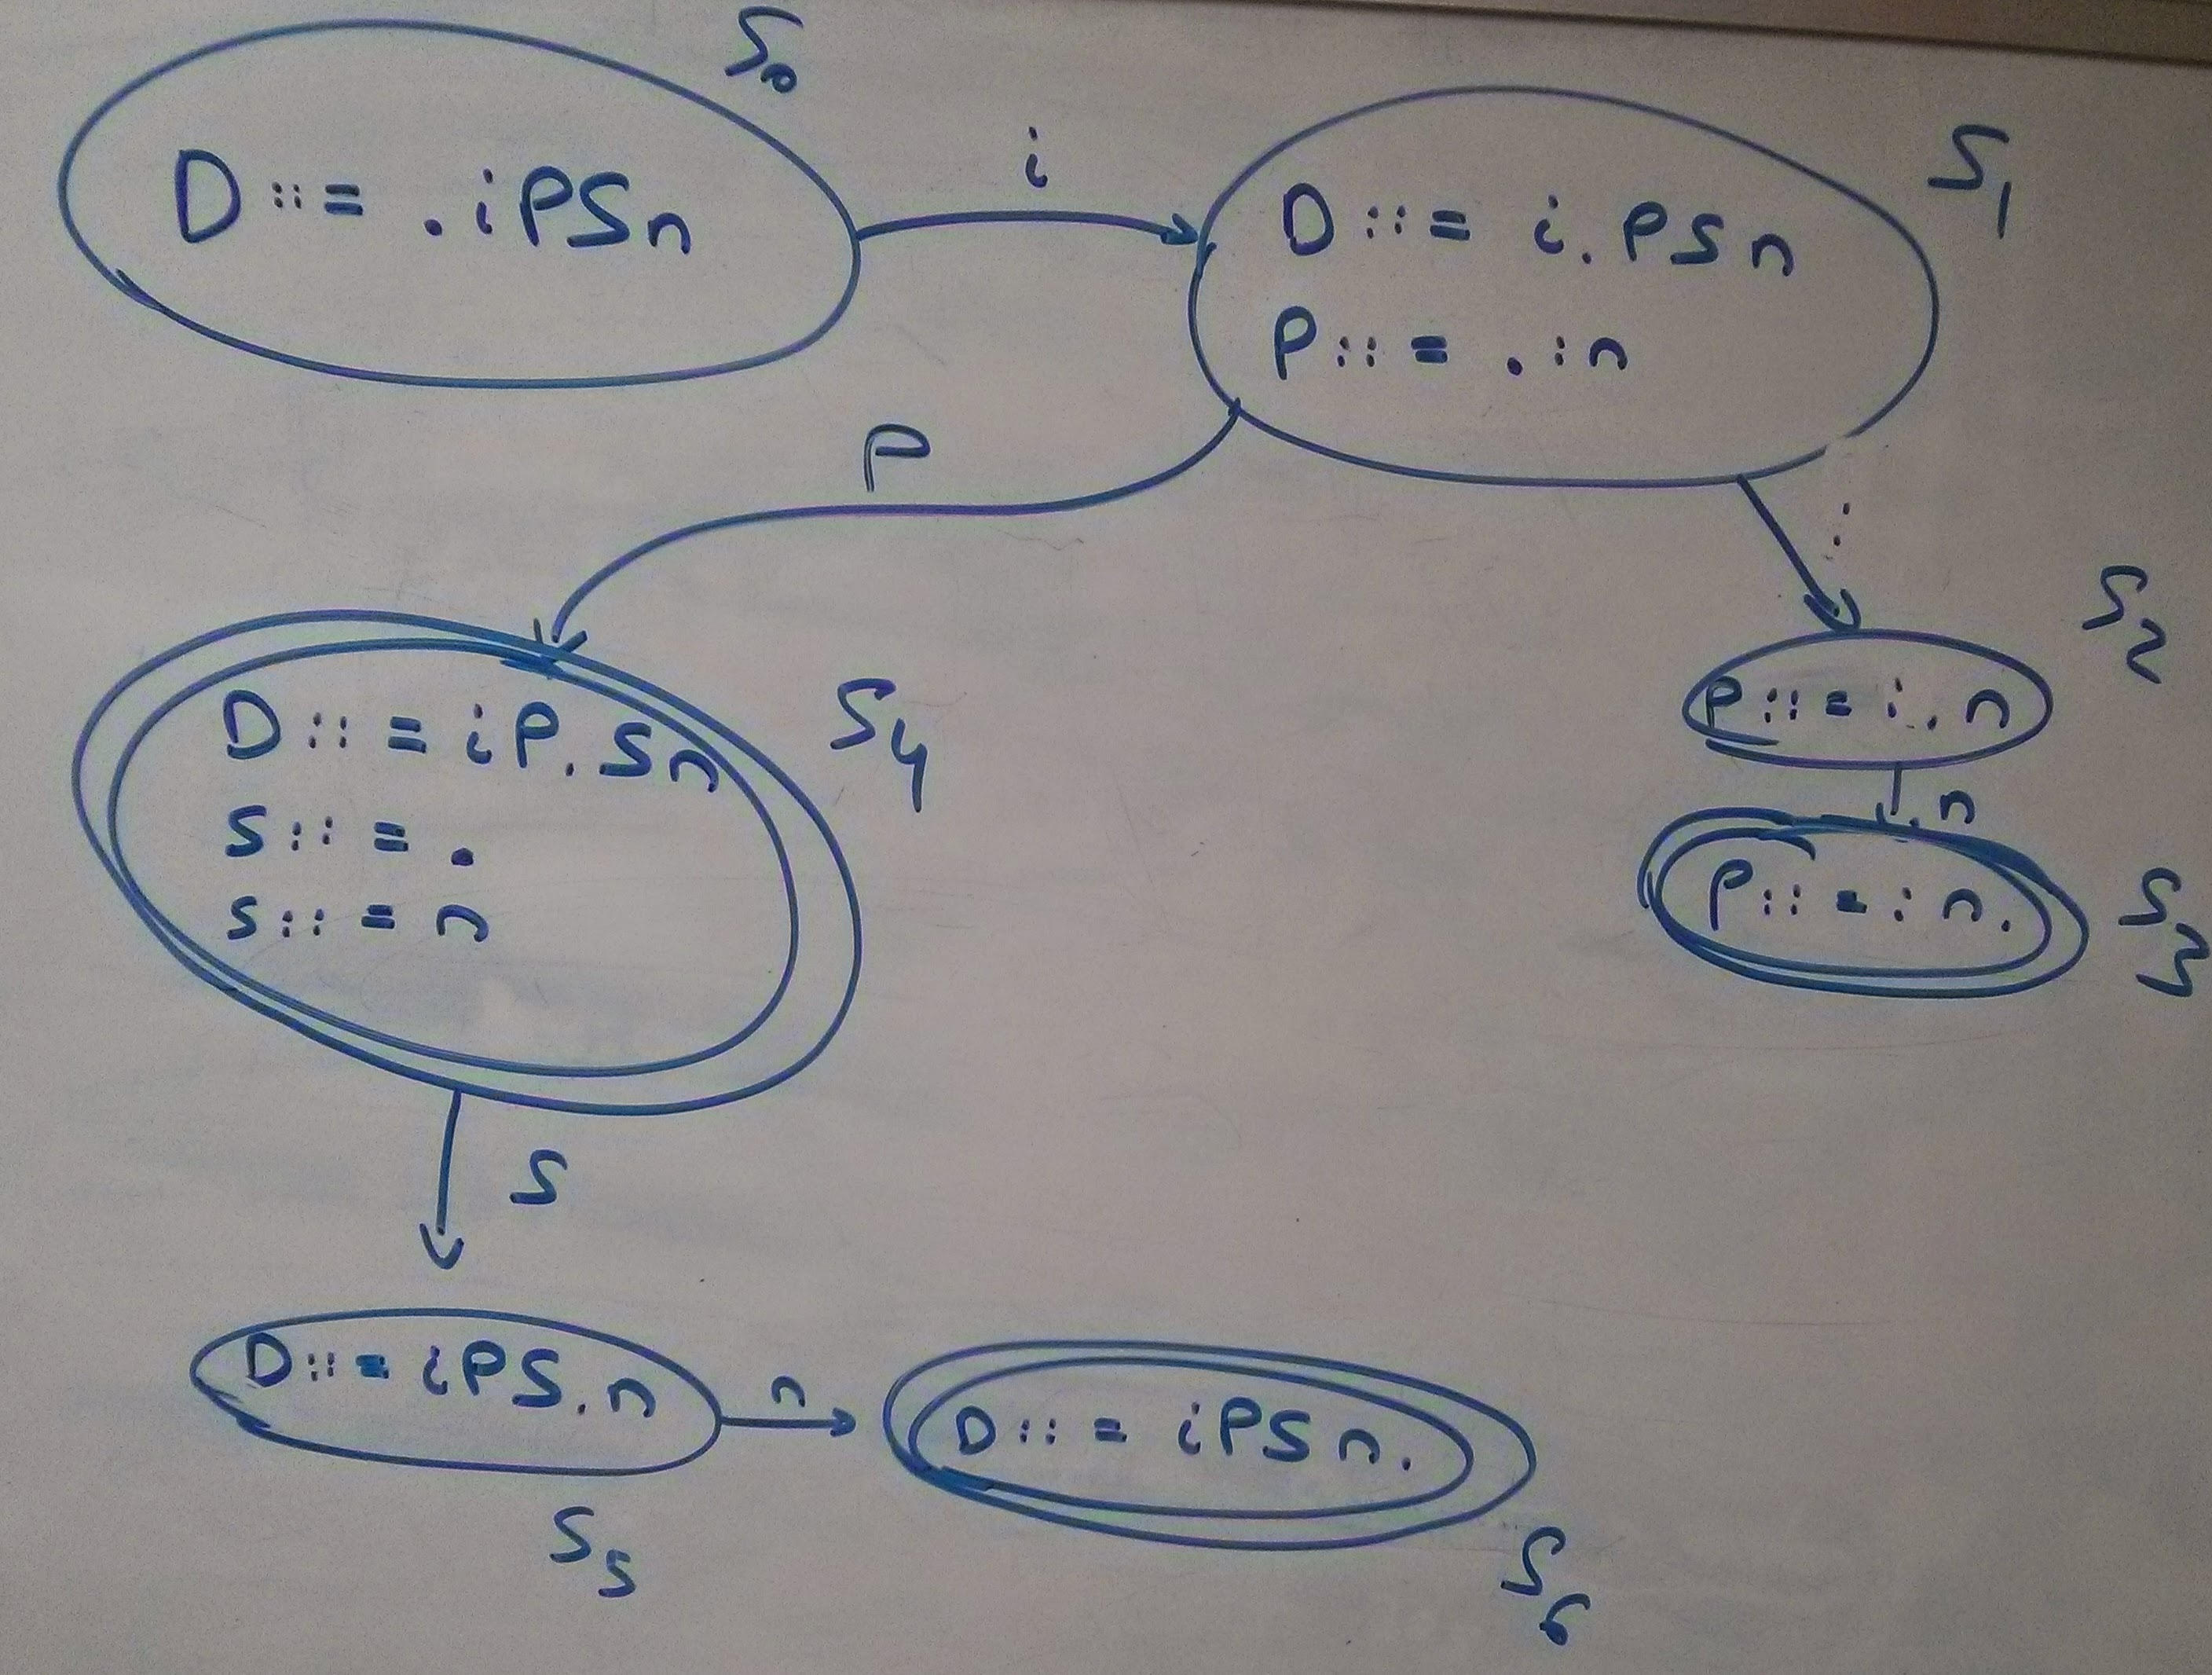
\includegraphics[scale=0.1]{peque.jpg}


\spart 

\begin{tabular}{c||c|c|c|c|c|c}
    & i & P & S & n & : & λ \\\hline\hline
$S_0$  &d1 &   &   &   &   &   \\\hline
$S_1$ &   &d4 &   &   & d2&   \\\hline
$S_2$ &   &   &   & d3&   &   \\\hline
$S_3$ & r2& r2& r2& r2& r2& r2\\\hline
$S_4$ & r3& r3& r3/d5& r3& r3& r3\\\hline
$S_5$ &   &   &   &d6 &   &   \\\hline
$S_6$ &r1 &r1 &r1 &r1 &r1 &r1 
\end{tabular}

\spart Esta gramática no es LR(0) porque presenta conflictos. 

Tampoco sería LR(1) debido a la regla λ, que hace imposible distinguir cuando reducir y cuándo desplazar.
\end{problem}
\newpage
\begin{problem}[5]
\ppart Dibuja el diagrama de estados del analizador LR(0) para dicha gramática.
\ppart Calcula la tabla de análisis para el analizador LR(0).
\ppart Indica justificadamente si la gramática es LR(0). Indica justificadamente si es
SLR(1).

\solution

\spart
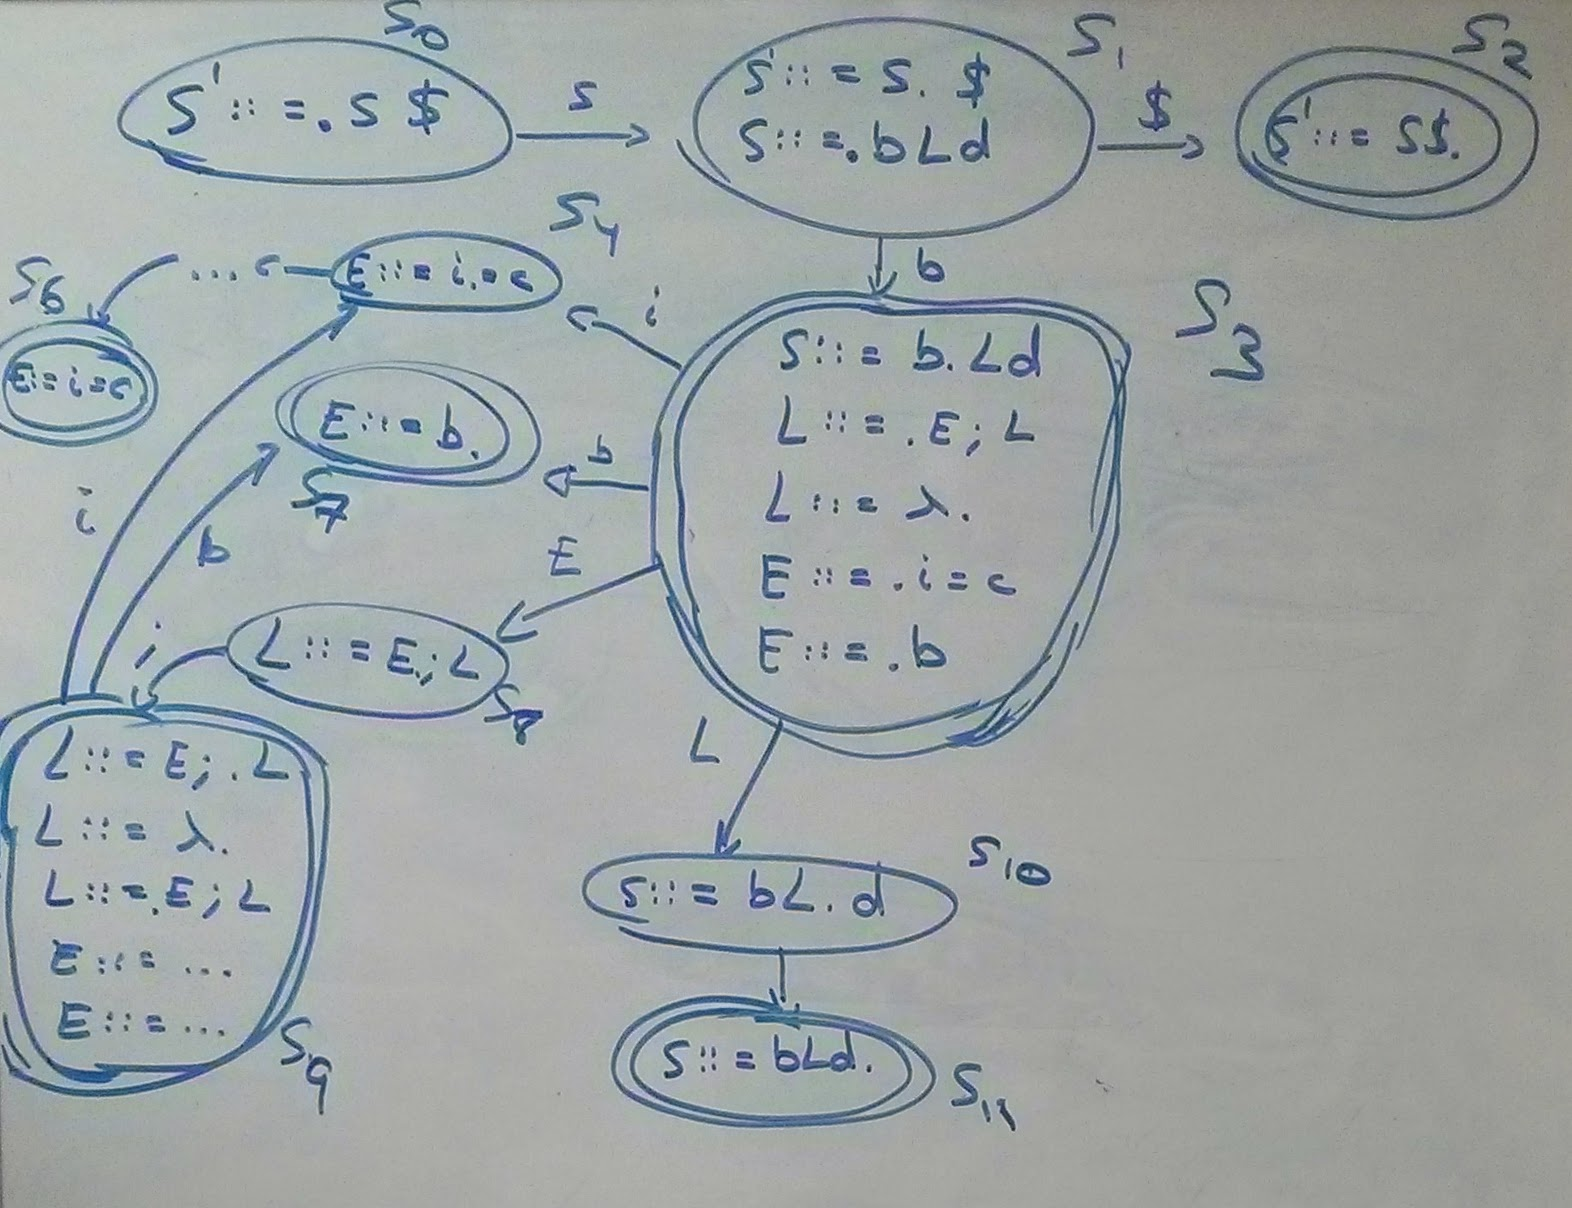
\includegraphics[scale=0.2]{grande.jpg}


\spart

\begin{tabular}{c||c|c|c|c|c|c|c|c|c|c}
   		&   S &  L &  E &  i &  = &  b &  c  &  d & λ  & \$\\
 $S_0$   &  d1&    &    &    &    &    &	 &	  &    &	\\\hline
 $S_1$   &    &    &    &    &    & d3 &    &	  &    & d2 \\\hline
 $S_2$   & r1 & r1 & r1 & r1 & r1 & r1 & r1 & r1 & r1 & r1 \\\hline
 $S_3$   &    & d10&  d8& d4 &    & d7 &	 &	  &    &	\\\hline
 $S_4$   &    &    &    &    & d5 &    &	 &	  &    &	\\\hline
 $S_5$   &    &    &    &    &    &    & d6 &	  &    &	\\\hline
 $S_6$   & r4 & r4 & r4 & r4 & r4 & r4 & r4 & r4 & r4 & r4 \\\hline
 $S_7$   & r5 & r5 & r5 & r5 & r5 & r5 & r5 & r5 & r5 & r5 \\\hline
 $S_8$   &    &    &    & d9 &    &    &    &    &    &    \\\hline
 $S_9$   & r3 & r3 & r3&r3/d4& r3&r3/d7& r3 & r3 & r3 & r3 \\\hline
$S_{10}$ &    &    &    &    &    &    &    &s11  &    &    \\\hline
$S_{11}$ & r11 & r11 & r11 & r11 & r11 & r11 & r11 & r11 & r11 & r11 \\\hline
\end{tabular}


\spart
Esta gramática no es LR(0) porque presenta conflictos. 

Tampoco sería LR(1) debido a la regla λ, que hace imposible distinguir cuando reducir y cuándo desplazar.

\end{problem}

\begin{problem}[6]

\solution
\begin{minipage}{0.3\textwidth}
\ppart
\begin{align*}
P(X)&=\{e,g\}\\
P(Y)&=\{g\}\\
P(Z)&=\{h\}\\
\end{align*}

\begin{align*}
S(X)&=\{\$\}\\
S(Y)&=\{\$,e,h\}\\
S(Z)&=\{\$,f\}\\
\end{align*}
\end{minipage}

\begin{minipage}{0.3\textwidth}
\ppart
\begin{align*}
P(X)&=\{c,i,f\}\\
P(Y)&=\{i,f\}\\
P(Q)&=\{f\}\\
\end{align*}
\begin{align*}
S(X)&=\{\$,i,f\}\\
S(Y)&=\{\$,i,f\}\\
S(Q)&=\{\$,i,f\}\\
\end{align*}
\end{minipage}

\begin{minipage}{0.3\textwidth}
\ppart

\begin{align*}
P(X)&=\{",",.,e\}\\
P(A)&=\{0,1,",",.,e\}\\
P(B)&=\{0,1,",",.,e\}\\
\end{align*}
\begin{align*}
S(X)&=\{\$,0,1\}\\
S(A)&=\{\$,\}\\
S(B)&=\{\$,",",.,e\}\\
\end{align*}
\end{minipage}

\end{problem}

\begin{problem}[7]
Calcula los símbolos de adelanto para el cierre de las siguientes reglas y gramáticas:
\ppart = Cierre de E’ ::= .E\{\$\} para la gramática:
\begin{gather*}
E’ ::= E\\
E ::= T\\
E ::= E+T\\
T ::= i\\
T ::= (E)\\
\end{gather*}
\ppart Cierre de S’ ::= .S \{\$\} para la gramática:
\begin{gather*}
S’ ::= S\\
S ::= L=R\\
S ::= R\\
L ::= *R\\
L ::= i\\
R ::= L\\
\end{gather*}
\ppart Cierre de E ::= (.L) \{\$\} para la gramática:
\begin{gather*}
E ::= (L)\\
E ::= a\\
L ::= L,E\\
L ::= E\\
\end{gather*}
\solution


\spart
\begin{align*}
E’ &::= .E&\{\$\}\\
E &::= .T &\{\$,+,( \}\\
E &::= .E+T &\{\$,+,(\}\\
T &::= .i &\{\$,+,(\}\\
T &::= .(E)&\{\$,+,(\}\\
\end{align*}

\spart


\begin{align*}
S’ &::= .S&\{\$\}\\
S &::= .L=R &\{\$,i\}\\
S &::= .R&\{\$\}\\
L &::= .*R &\{=\}\\
L &::= .i \{=\} \\
R &::= .L \{=\} \\
\end{align*}


\spart

\begin{align*}
E &::= (.L) &\{\$\}\\
L &::= .L,E &\{\$\}\\
L &::= .E&\{\$,','\}\\
E &::= .a&\{')',\$ \}  \\
\end{align*}
\end{problem}


\end{document}